%%PREAMBLE %%%%%%%%%%%%%%%%%%%%%%%%%%%%
\documentclass[10pt, a4paper]{article}% size of txt = 10pt
\usepackage[top= 2cm,
			bottom = 2cm,
			left = 1.7cm,
			right = 1.7cm,
			footskip = 0.5cm,
			headsep = 0cm,
			headheight = 0cm
					]{geometry}
\usepackage{amsmath} % math packages
\usepackage{amsfonts}% math packages
\usepackage{amssymb} % math packages
\usepackage{graphicx} %package for including graphics
\usepackage{array}
\usepackage[thinlines]{easytable}
\usepackage{float}
\usepackage[section]{placeins}
\usepackage[hidelinks]{hyperref}
\usepackage[shortlabels]{enumitem}
\usepackage{svg}
\usepackage{bigstrut}
\usepackage{wrapfig,lipsum,booktabs}
\usepackage{subcaption}
\usepackage{xfrac}
\usepackage{pdfpages}
\usepackage{listings}
\usepackage{xcolor}

\usepackage{listings}
\usepackage{color} %red, green, blue, yellow, cyan, magenta, black, white
\definecolor{mygreen}{RGB}{28,172,0} % color values Red, Green, Blue
\definecolor{mylilas}{RGB}{170,55,241}

\definecolor{codegreen}{rgb}{0,0.6,0}
\definecolor{codegray}{rgb}{0.5,0.5,0.5}
\definecolor{codepurple}{rgb}{0.58,0,0.82}
\definecolor{backcolour}{rgb}{1,1,1}

\lstdefinestyle{mystyle}{
    backgroundcolor=\color{backcolour},   
    commentstyle=\color{codegreen},
    keywordstyle=\color{magenta},
    numberstyle=\tiny\color{codegray},
    stringstyle=\color{codepurple},
    basicstyle=\ttfamily\footnotesize,
    breakatwhitespace=false,         
    breaklines=true,                 
    captionpos=b,                    
    keepspaces=true,                 
    numbers=left,                    
    numbersep=5pt,                  
    showspaces=false,                
    showstringspaces=false,
    showtabs=false,                  
    tabsize=2
}
\lstset{style=mystyle}


%date format
\def\mydate{\leavevmode\hbox{\twodigits\day.\twodigits\month.\the\year}}
\def\twodigits#1{\ifnum#1<10 0\fi\the#1}


\usepackage[T1]{fontenc} 
\usepackage{lmodern}
\usepackage{indentfirst}
\setlength{\parindent}{1cm}

\makeatletter
\newcommand{\thickhline}{%
    \noalign {\ifnum 0=`}\fi \hrule height 2pt
    \futurelet \reserved@a \@xhline
}
\newcolumntype{"}{@{\hskip\tabcolsep\vrule width 2pt\hskip\tabcolsep}}
\makeatother
\newcolumntype{?}{!{\vrule width 2pt}}
%%DOC ENVIROMENT%%%%%%%%%%%%%%%%%%%%%%%
\begin{document}
%Title 
\begin{flushleft}%% left justification
	\textbf{\Large{MKC-KBC: Úkol č. 4}}\hfill Filip Paul\\
	\large{koaxiání monopól v blízkosti lidských zad \hfill\mydate}
\end{flushleft}

\section{\Large Model jednoho monopólu:}
\begin{figure}[ht!]
	\centering
	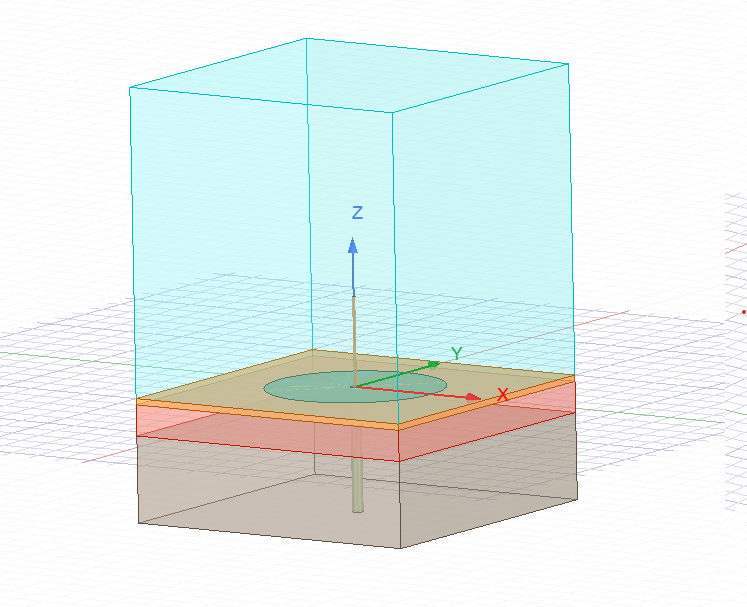
\includegraphics[height = 0.3\textheight]{single_model.png}
	\captionof{figure}{3D model zkoumaného monopólu v blízkosti lidské tkáně}
\end{figure}

	\begin{figure}[ht!]
		\centering
		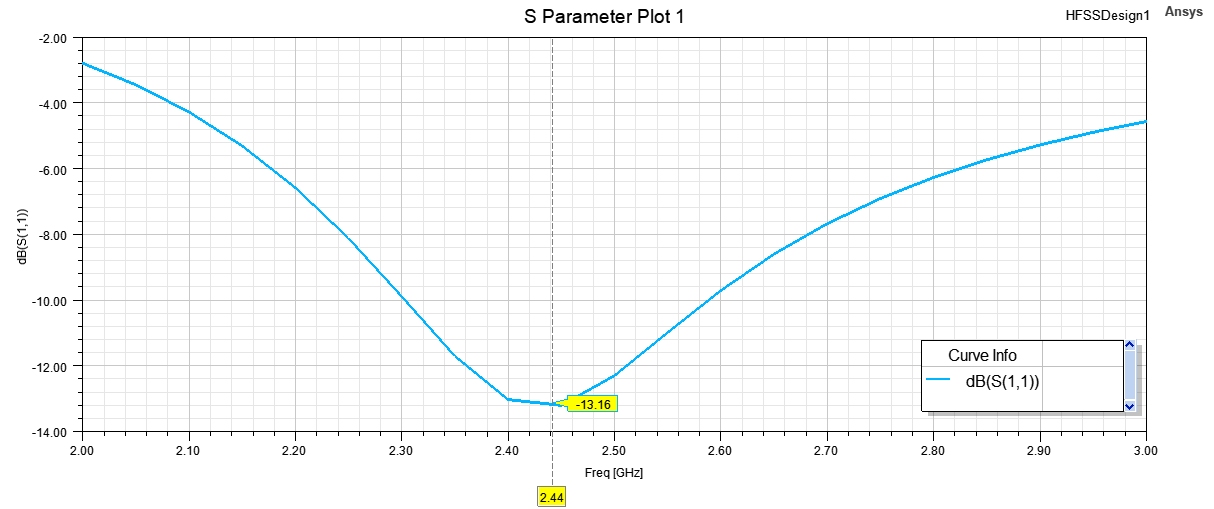
\includegraphics[width = 1\textwidth,height = 0.4\textheight]{S11.png}
		\captionof{figure}{S11 parametr}
	\end{figure}
Pro zvolenou délku monopólu ant\_l = 19mm. Lze z z grafu pro S11 parametry určit rezonanční kmitočet
přibližně 2.45 GHz. 
\clearpage
\begin{figure}[ht!]
	\centering
	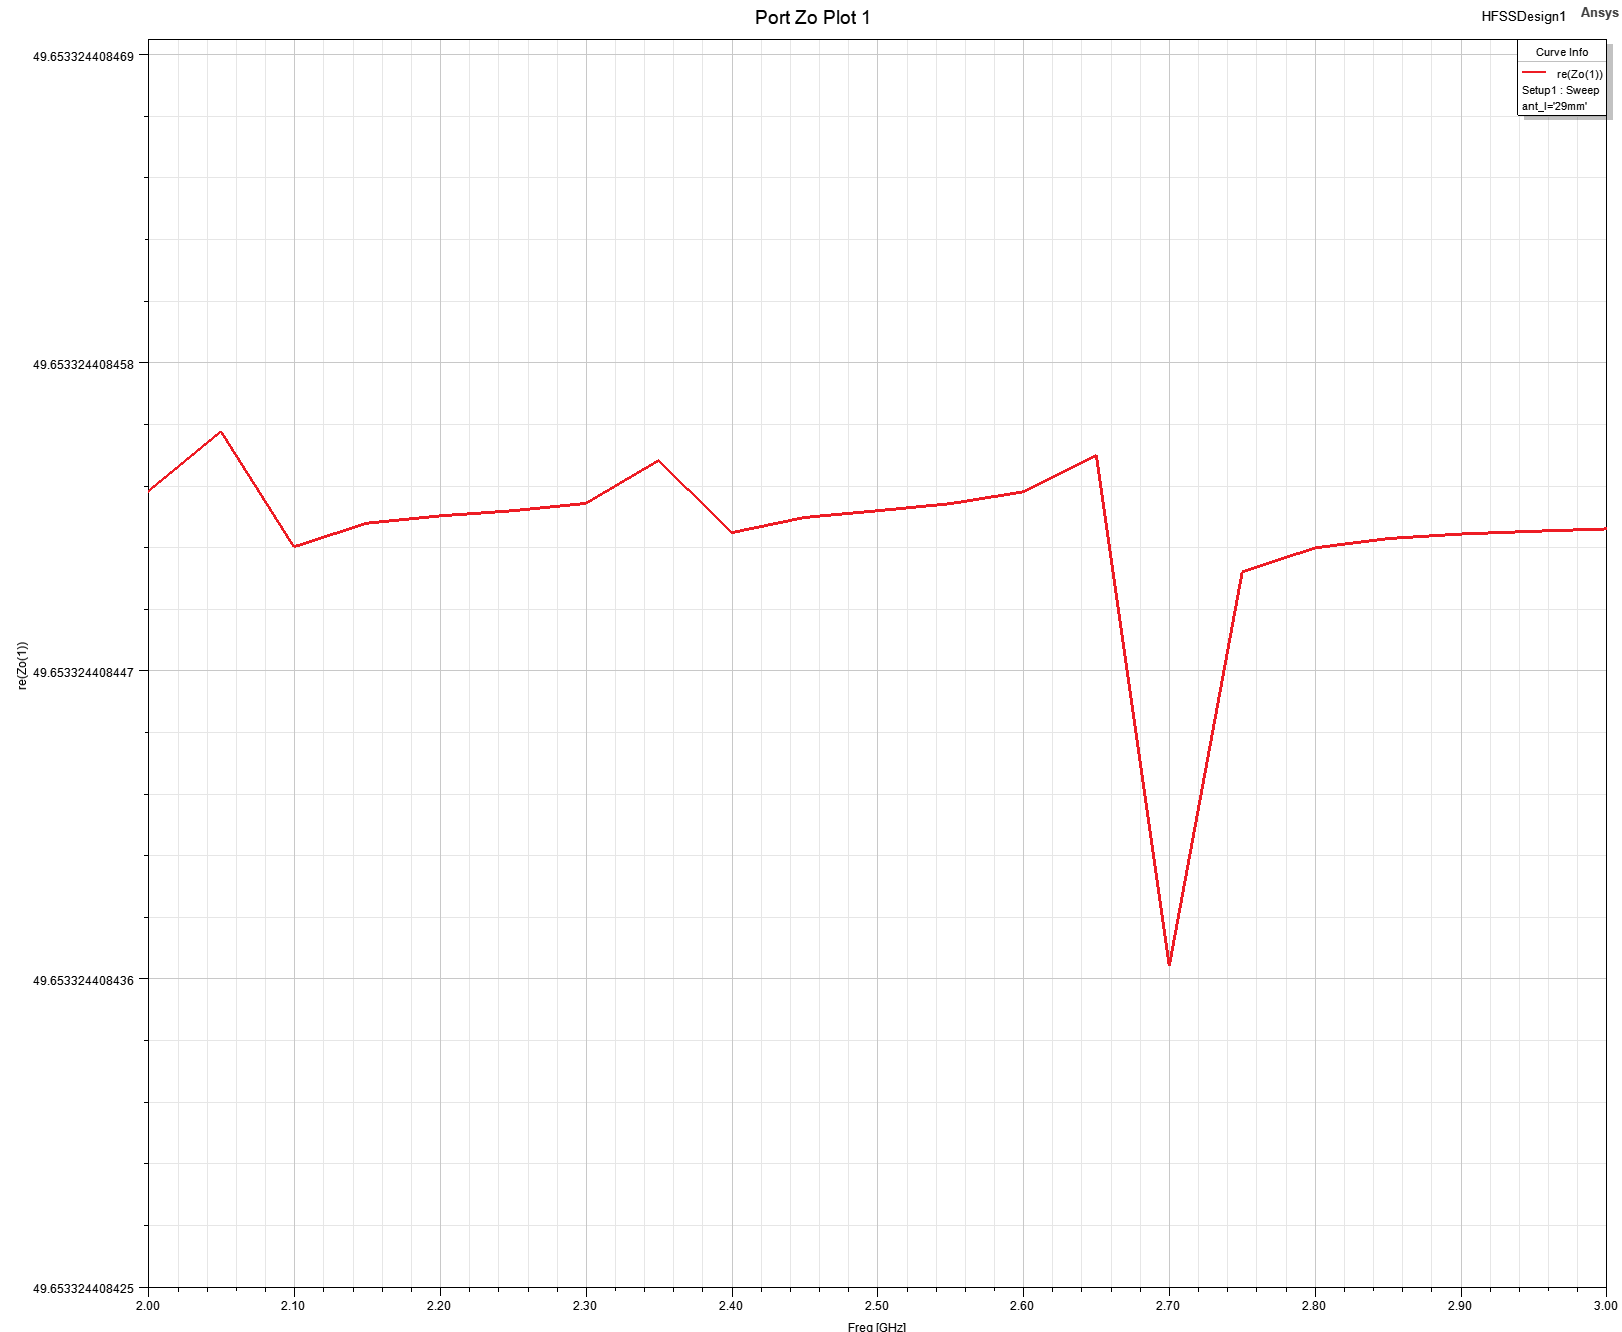
\includegraphics[width = 1\textwidth]{Z0.png}
	\captionof{figure}{Charakteristická impedance koaxiálního kabelu}
\end{figure}
Cílem bylo navrhnout připojení pomocí koaxiálního kabelu s charakteristickou impedancí Z0 = 50 Ohm.
Chyba v celém rozsahu kmitočtů nepřesahuje 1$\Omega$.

\begin{figure}[ht!]
	\centering
	\begin{minipage}{.45\textwidth}
		\centering
		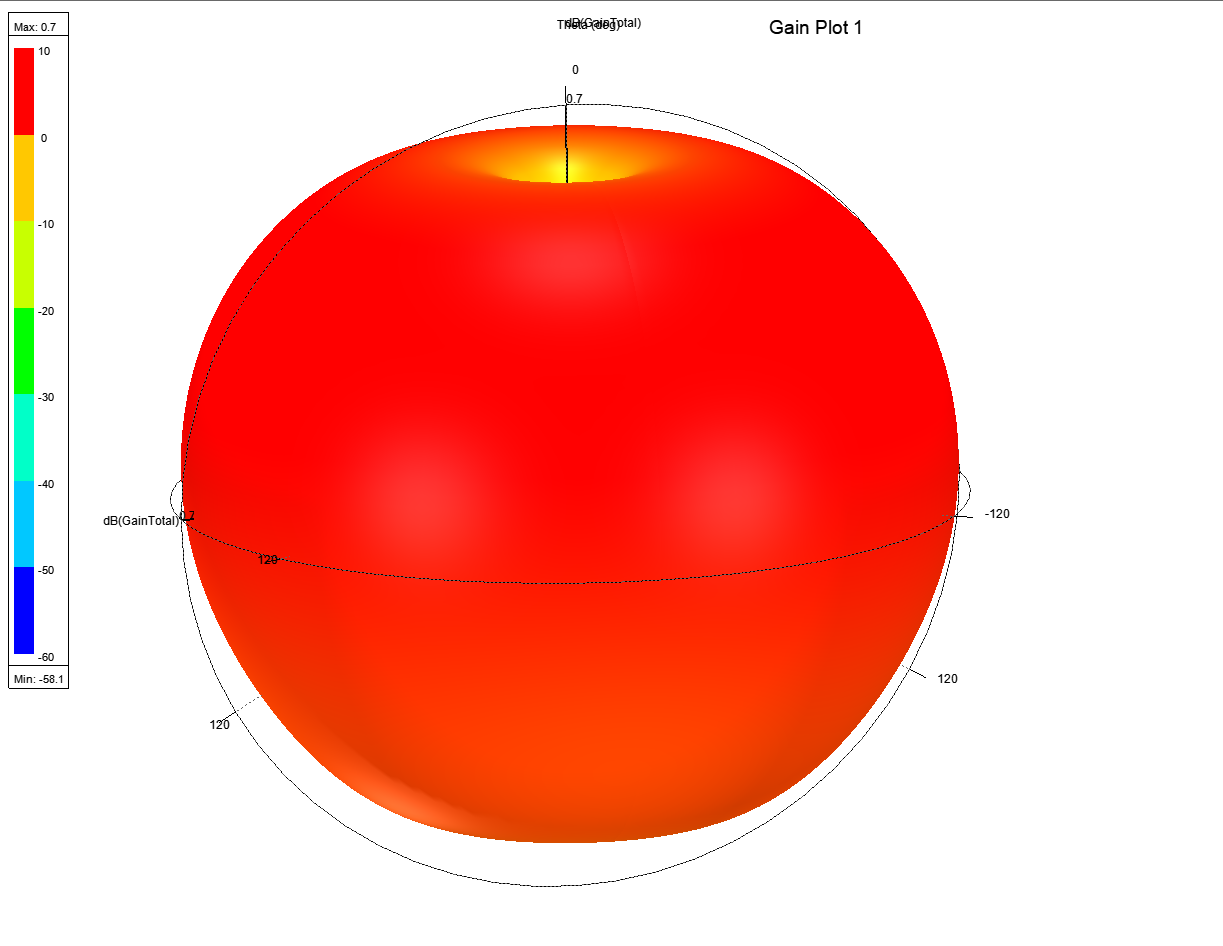
\includegraphics[height = 0.3\textheight]{log_scale.png}
		\captionof{figure}{Vyzařování ve vzdáleném poli v případě pouze jedné antény - zisk je v lineárních jednotkách}
	\end{minipage}%
	\hfill
	\begin{minipage}{.45\textwidth}
		\centering
		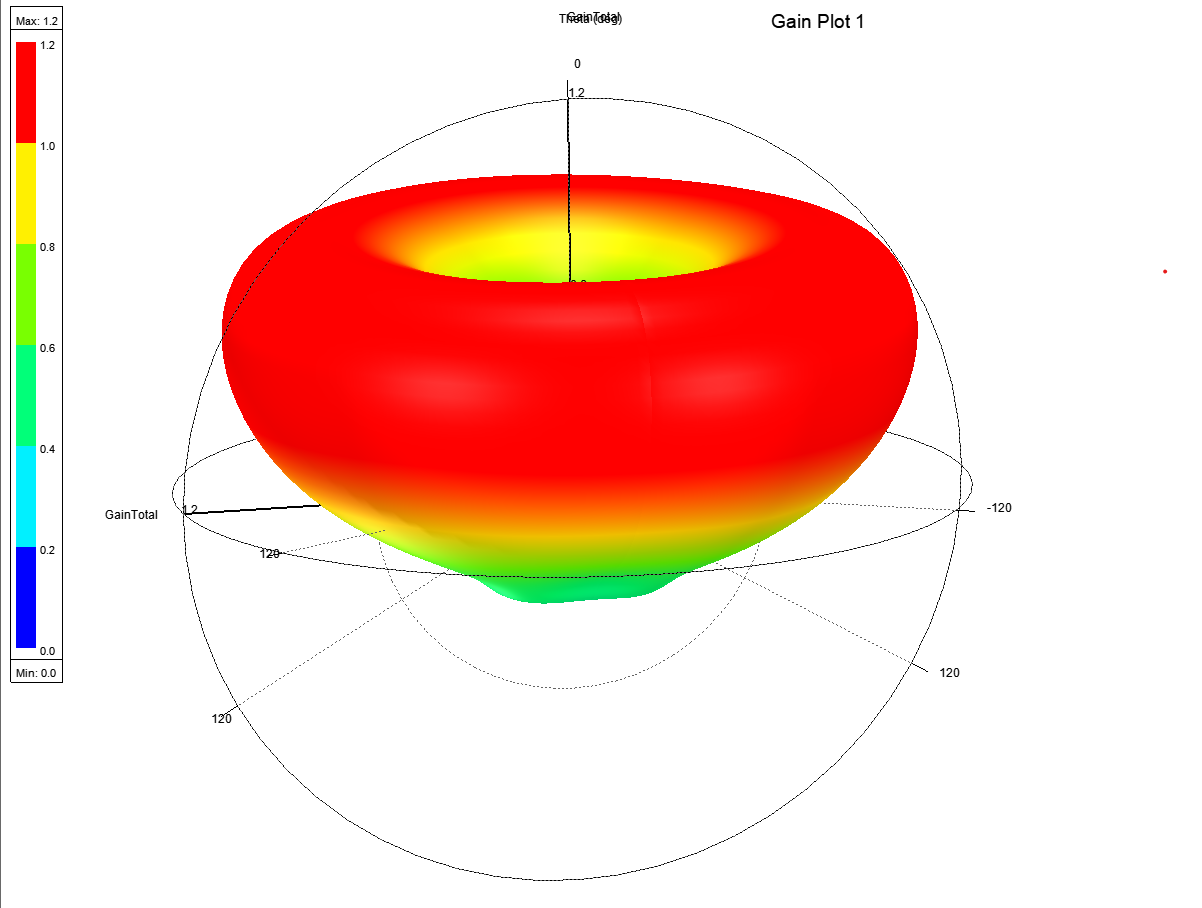
\includegraphics[height = 0.3\textheight]{normal_scale.png}
		\captionof{figure}{Vyzařování ve vzdáleném poli v případě obou antén - zisk je v lineárních jednotkách}
	\end{minipage}
	\end{figure}

Vzhledem k nízkému zisku monopólu jsou vyzařovací charakteristiky v lineárních jednotkách, aby byl
na první pohled patrnější vliv reflektoru a ztrát ve fantomu. V případě simulace s oběma anténami došlo k deformaci
vyzařovací charakteristiky. 


\clearpage

\section{\Large "Full"  a "Symetry" model dvojice monopólů poblíž lidských zad}
\begin{figure}[ht!]
	\centering
	\begin{minipage}{0.45\textwidth}
		\centering
		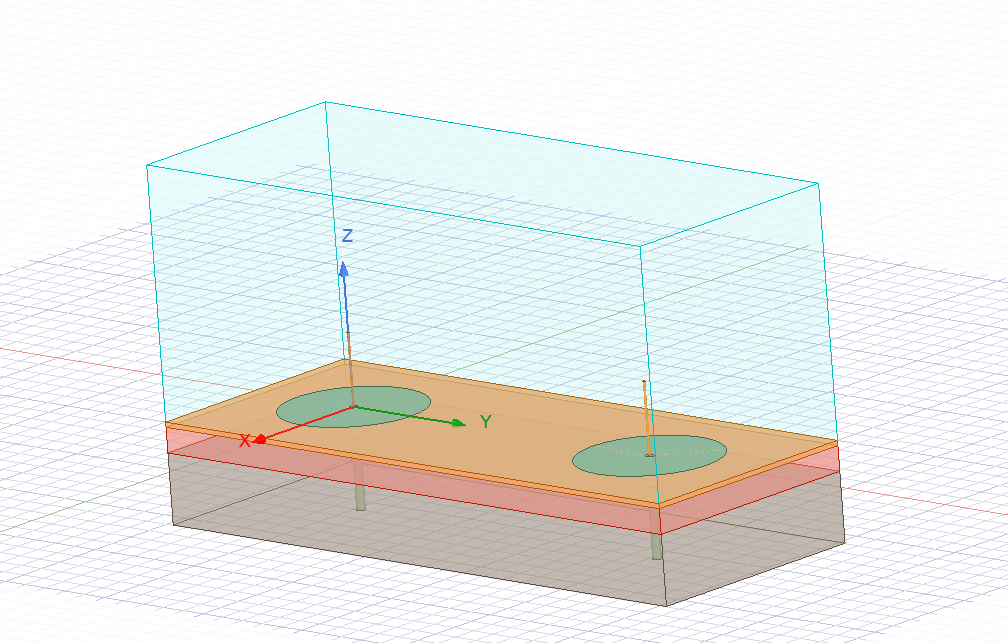
\includegraphics[width= 1\textwidth, height = 0.25\textheight]{dual_model.png}
		\captionof{figure}{3D - "Full" Model dvojice monopólů v blízkosti lidských zad}
	\end{minipage}%
	\hfill
	\begin{minipage}{0.45\textwidth}
		\centering
		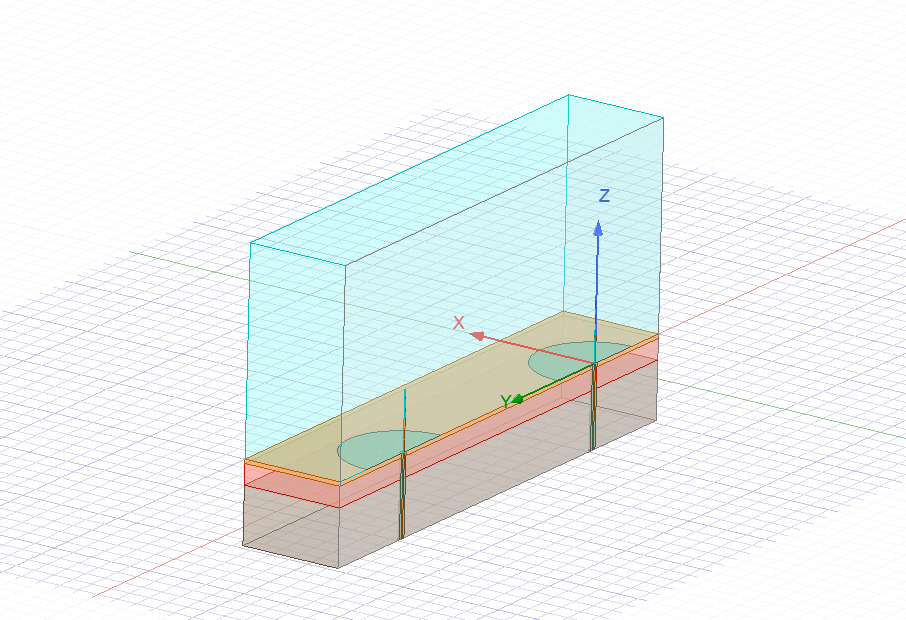
\includegraphics[width= 1\textwidth,height = 0.25\textheight]{symetry_model.png}
		\captionof{figure}{3D - "Symetry" Model dvojice monopólů v blízkosti lidských zad}
	\end{minipage}
	\end{figure}

Předpokladem je, že by "Symetry" model měl mít výrazně nižší výpočetní náročnost oproti "Full" modelu.
Následující tabulky zobrazují celkový čas simulace v případě použití "FULL" a "Symetry" modelů. Úspora
času simulace v případě "Symetry" modelu je přibližně 60\%. Nicméně ANSYS defaultně omezuje
maximální prostředky hardwaru použitého k simulaci. V případě použití defaultního nastavení
trvala simulace "FULL" modelu přibližně 12 min. Po povolení používat pro simulaci vyšší míru hardwarových
prostředků bylo dosaženo celkovému času simulace "FULL" modelu 01:46. Před každou simulací byla vymazána
všechny odsimulovaná data, aby byl solver donucen k novému výpočtu všech simulačních dat.

\begin{figure}[ht!]
	\centering
	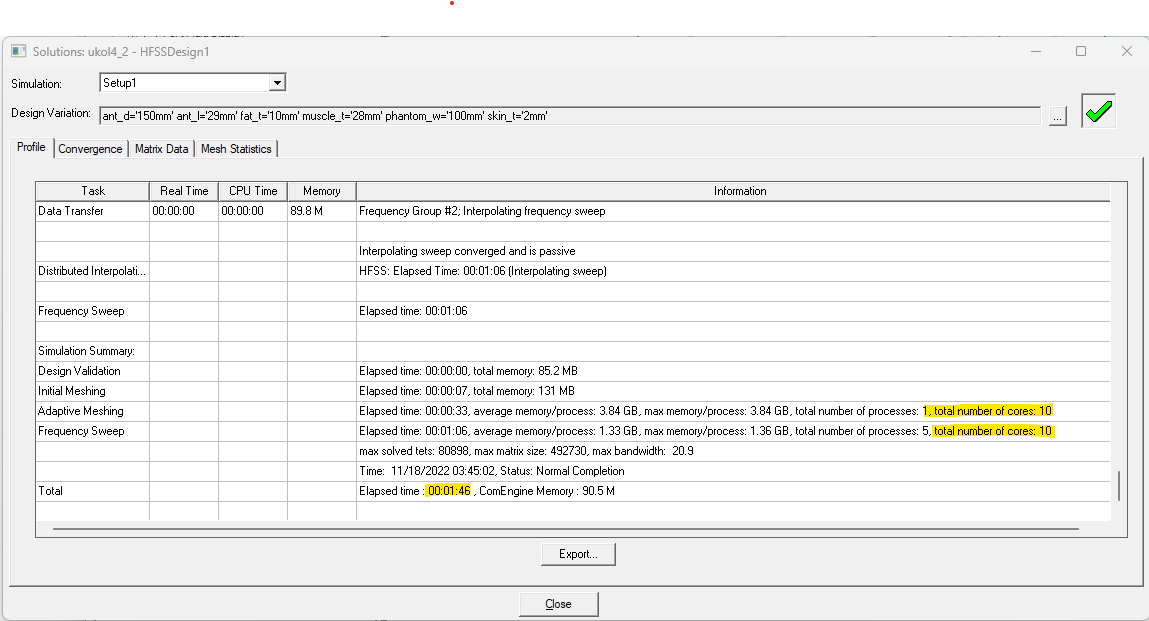
\includegraphics[width = 1\textwidth]{elapsed_time_full.png}
	\captionof{figure}{celkový čas analýzy za použití "full" modelu}
\end{figure}
\clearpage

\begin{figure}[ht!]
	\centering
	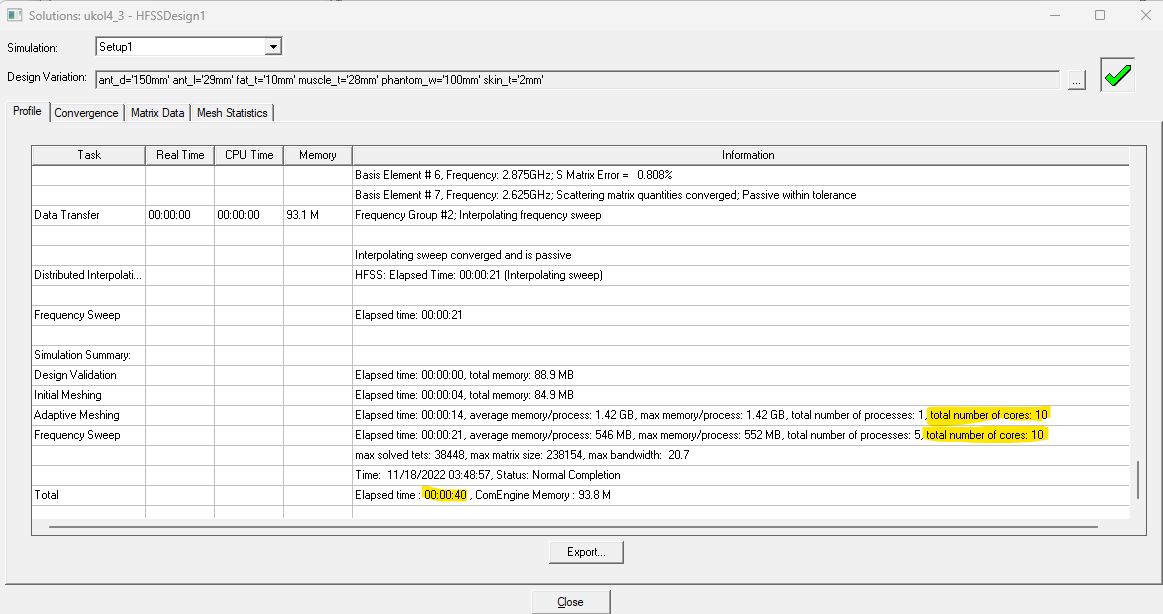
\includegraphics[width = 1\textwidth]{elapsed_time_symetry.png}
	\captionof{figure}{celkový čas analýzy za použití "Symetry" modelu}
\end{figure}

V obrázcích (11 a 12),je patrné, že se výsledné hodnoty simulace pro "Symetry" a "Full" modely liší.
"Full" model by měl být přesnější a tak je vhodné na konci návrhu ověřit výsledky simulace za použití
právě "Full" modelu za cenu vyšší časové náročnosti simulace.

\begin{figure}[ht!]
	\centering
	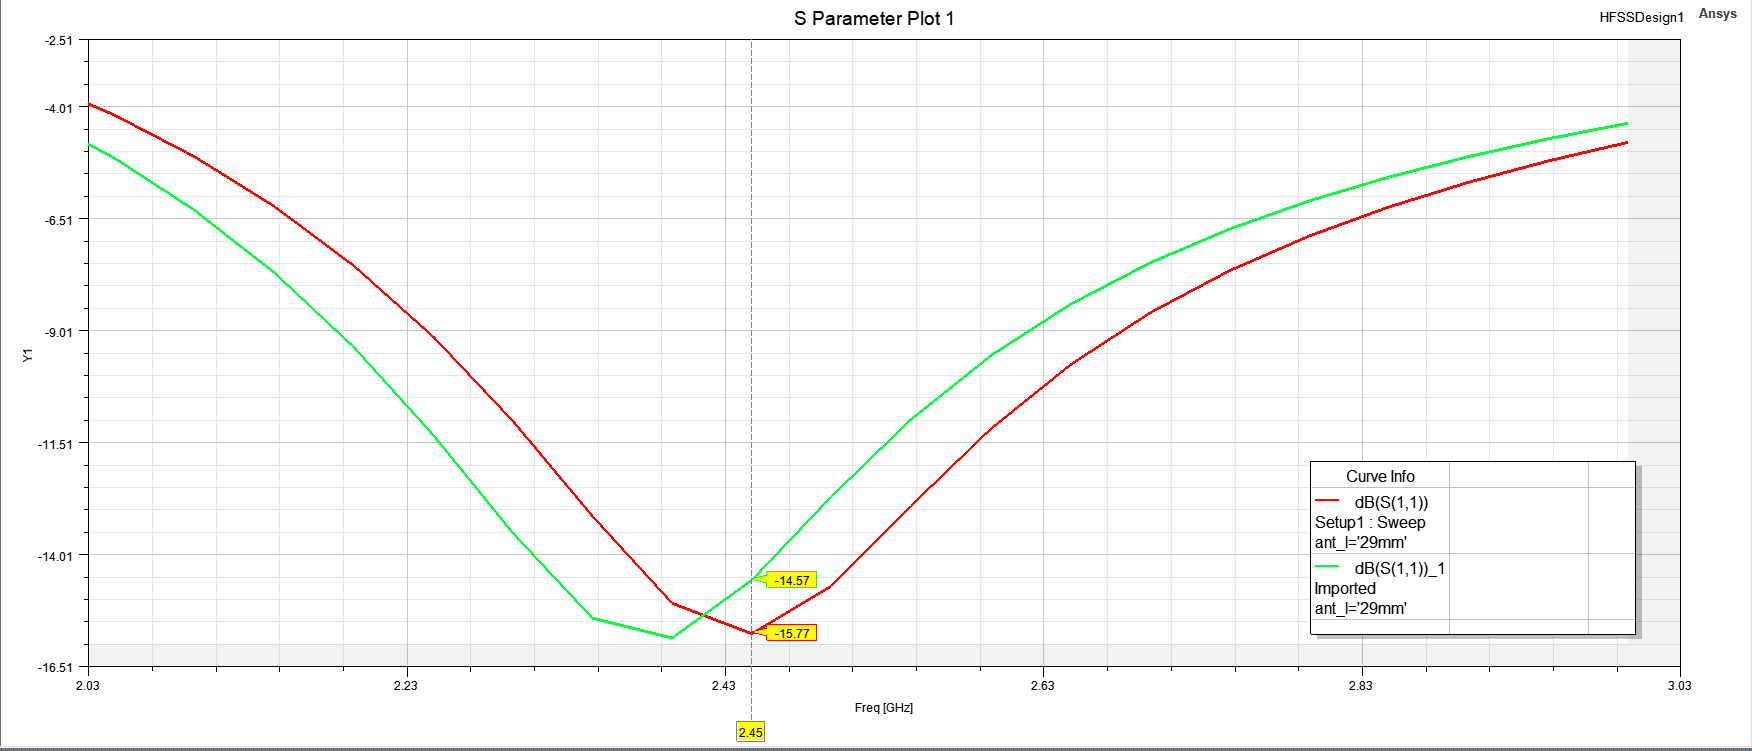
\includegraphics[height = 0.26\textheight,width = 1\textwidth]{S11_compare.png}
	\captionof{figure}{Porovnání S11 parametru při použití "full" (zeleně) a "Symetry" (červeně)  modelu}
\end{figure}
\clearpage

\begin{figure}[ht!]
	\centering
	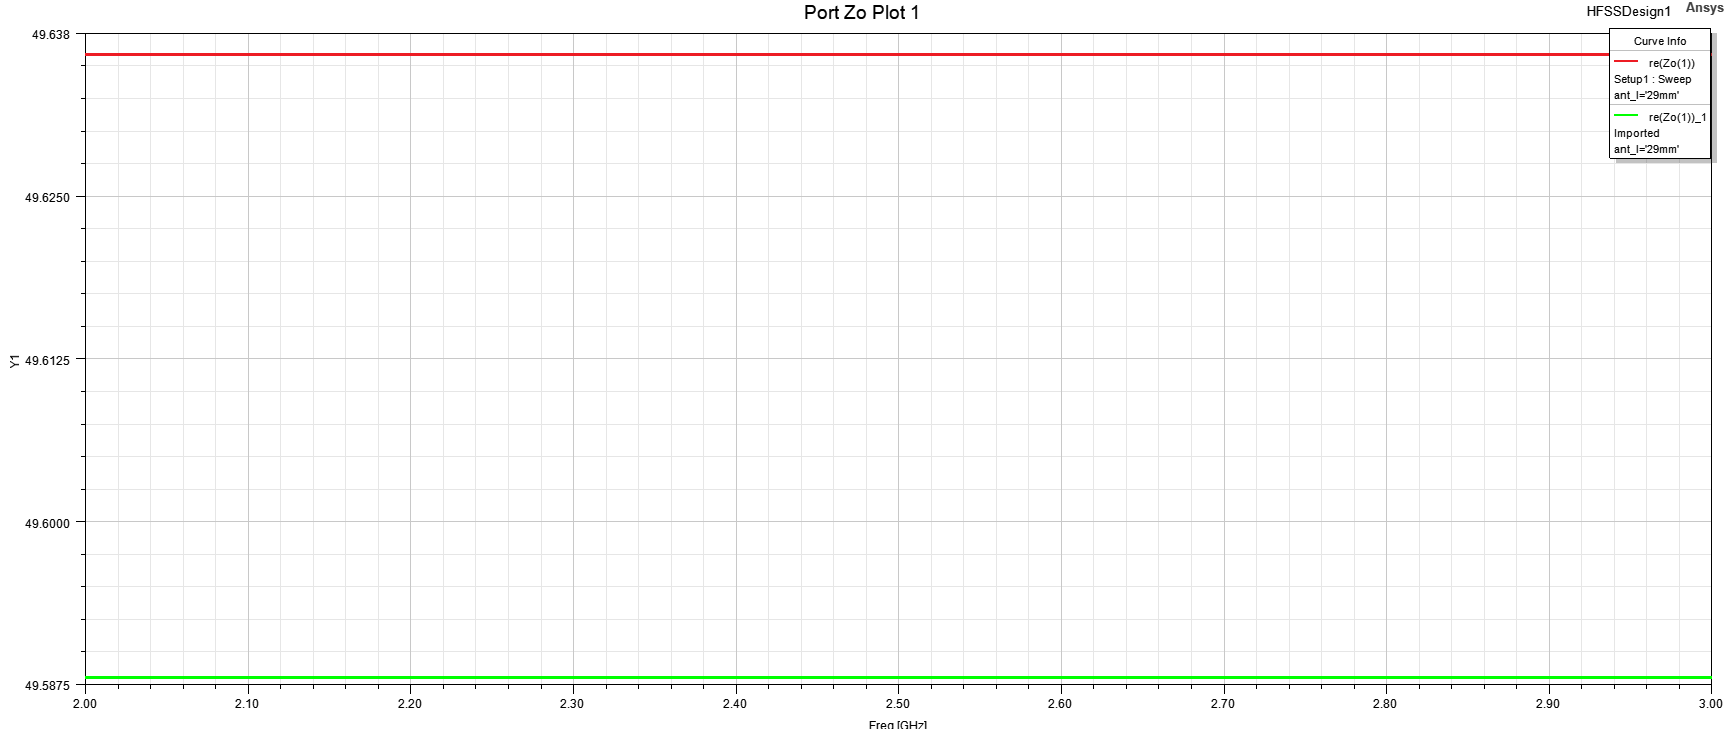
\includegraphics[height = 0.26\textheight,width = 1\textwidth]{Z0_compare.png}
	\captionof{figure}{Porovnání char. impedance Z0 při použití "full" (červeně) a "Symetry" (zeleně)  modelu}
\end{figure}

Obrázek níže znázorňuje rozložení elektrického pole při dané fázi buzení monopólu. V animaci (v prostředí ANSYS),
lze pozorovat jak se mění elektrické pole jedné antény v závislosti na buzení antény druhé. Lze tak předpokládat,
že je možno mezi anténami komunikovat. Zároveň jde vidět, že se elektrické pole šíří především ve volném prostředí
charakterizovaným vakuem a pouze malá část radiace je přenášena lidskými tkáněmi.
\begin{figure}[ht!]
	\centering
	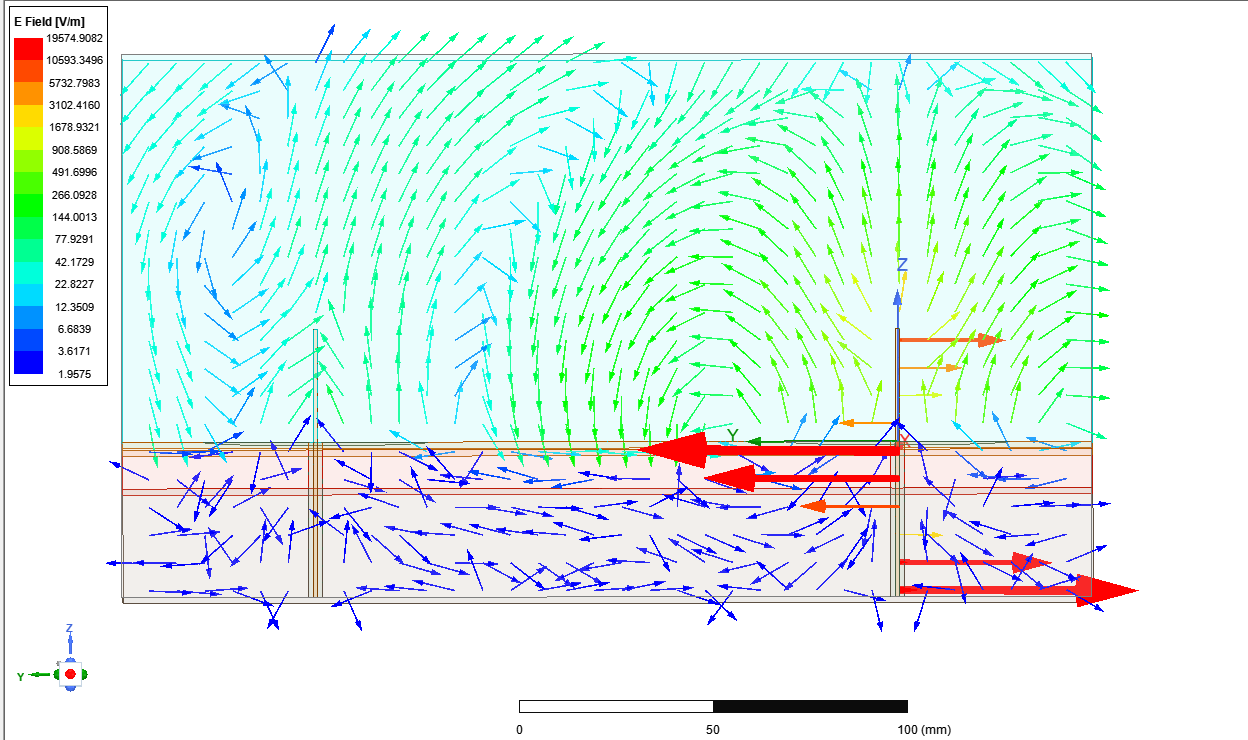
\includegraphics[height = 0.3\textheight,width = 1\textwidth]{E_field_symetry.png}
	\captionof{figure}{E-field v "symetry" modelu}
\end{figure}

\begin{figure}[ht!]
	\centering
	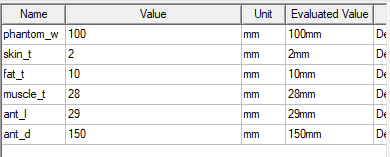
\includegraphics[height = 0.1\textheight]{variables.png}
	\captionof{figure}{Parametry simulace}
\end{figure}


\end{document}

%\[f(x)= (x+2)^2 - \frac{9\cdot 2\pi}{26}\] %%mathematic equatation in display style mode
%%optional:
%	\begin{align} %%this alignes all charakters after & if *is removed equations will be numbered
%	\hspace{5cm}  
%		 x &= a_2 x^2 +_1 x + a_0 \\
% 		x &=x^2 \nonumber		%no number will not add number to eq
%	\end{align}
